\documentclass{article}

% if you need to pass options to natbib, use, e.g.:
% \PassOptionsToPackage{numbers, compress}{natbib}
% before loading nips_2016
%
% to avoid loading the natbib package, add option nonatbib:
% \usepackage[nonatbib]{nips_2016}

% \usepackage{nips_2016}

% to compile a camera-ready version, add the [final] option, e.g.:
\usepackage[final]{nips_2016}

\usepackage[utf8]{inputenc} % allow utf-8 input
\usepackage[T1]{fontenc}    % use 8-bit T1 fonts
\usepackage{hyperref}       % hyperlinks
\usepackage{url}            % simple URL typesetting
\usepackage{booktabs}       % professional-quality tables
\usepackage{amsfonts}       % blackboard math symbols
\usepackage{nicefrac}       % compact symbols for 1/2, etc.
\usepackage{microtype}      % microtypography

\usepackage{graphicx}
\usepackage{caption}

\title{Reading Summary 1 - HMOG: New Behavioral Biometric Features for Continuous Authentication of Smartphone Users}

\author{
  John Kath \\
  \texttt{john.kath@cgu.edu} \\
}

\begin{document}

\maketitle

% \begin{abstract}
% \end{abstract}

\section{HMOG Paper Summary}

NOTE: Reading summary is a restatement of material from reference [1].

\subsection{Description}

The authors introduce {\em Hand Movement, Orientation, and Grasp} (HMOG), a set of behavioral features to continuously authenticate smartphone users. HMOG features unobtrusively capture subtle micro-movement and orientation dynamics resulting from how a user grasps, holds, and taps on the smartphone.

Data from 100 subjects was collected under two conditions: sitting and walking. Authentication EERs as low as 7.16\% (walking) and 10.05\% (sitting) were achieved with combined HMOG, tap, and keystroke features. Experiments to investigate why HMOG features perform well during walking were conducted.

With BKG (Bimetric Key Generation), the authors achieved EERs of 15.1\% using HMOG combined with taps. In comparison, BKG using tap, key hold, and swipe features had EERs between 25.7\% and 34.2\%.

\subsection{Introduction}

In this paper, the authors present Hand Movement, Orientation, and Grasp (HMOG), a new set of behavioral biometric features for continuous authentication of smartphone users. HMOG uses accelerometer, gyroscope, and magnetometer readings to unobtrusively capture subtle hand micro-movements and orientation patterns generated when a user taps on the screen. 

Motivated by the above, they designed 96 HMOG features and evaluated their {\em continuous user authentication} and {\em biometric key generation} performance during typing. Because walking has been shown to affect typing performance, they evaluated HMOG under both walking and sitting conditions. 

\paragraph{New HMOG Features for Continuous Authentication} 
Two types of HMOG features are proposed: {\em resistance features}, which measure the micro-movements of the phone in response to the forces exerted by a tap gesture; and {\em stability features}, which measure how quickly the perturbations in movement and orientation, caused by tap forces, dissipate. %

\paragraph{Empirical Investigation Into Why HMOG Authentication Performs Well During Walking}  HMOG features achieved lower authentication errors (13.62\% EER) for walking compared to sitting (19.67\% EER). The authors investigated why HMOG had superior performance during walking by comparing the performance of HMOG features {\em during} taps and {\em between} taps (i.e., the segments of the sensor signal that lie between taps). Results suggest that the higher authentication performance %
during walking can be attributed to the ability of HMOG features to capture distinctive 
%
movements caused by walking in addition to micro-movements caused by taps. %

\paragraph{BKG with HMOG Features} 
%
BKG is closely related to authentication, but has a different objective: to 
provide cryptographic access control to sensitive data on the smartphone. Because the adversary is usually assumed to have physical access to the device, cryptographic keys must not be stored on the smartphone's memory---but rather generated from biometric signals and/or passwords.

Results on BKG can be summarized as follows: the authors achieved lower EERs with HMOG features compared to key hold, tap, and swipe features in both walking and sitting conditions. For walking, EER of HMOG-based BKG was 17\%, vs. 29\% with key hold and 28\% with tap features. By combining HMOG and tap features, the authors achieved 15.1\% EER. For sitting, an EER of 23\% with HMOG features, 26\% with tap features, and 20.1\% by combining both. In contrast, an ERR of 34\% was obtained with swipes.

\paragraph{Energy Consumption Analysis of HMOG Features}
Analysis shows that a balance between authentication performance and energy overhead can be achieved by sampling HMOG features at 16Hz. The energy overhead with 16Hz is 7.9\%, compared to 20.5\% with 100Hz sampling rate, but comes with minor increase (ranging from 0.4\% to 1.8\%) in EERs.

\begin{figure}[t]
  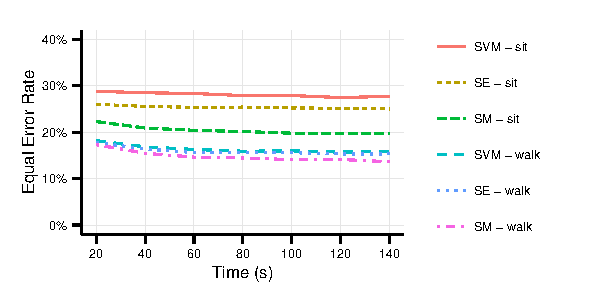
\includegraphics[width=1\linewidth]{plots_R/auth_hmog_all_verifiers_new.pdf}
  \caption[]{Comparison of HMOG features in sitting and walking conditions for three verifiers. The reported EERs are with PCA for SE, and for SVM-sitting; and without PCA for SM and SVM-walking. $X$-axis shows authentication time in seconds.}
  %
  \label{fig:hmogAllVerifiersSitWalk}
\end{figure}
  
\begin{figure}[t]
  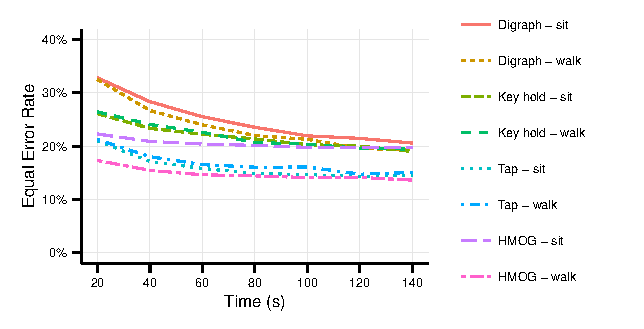
\includegraphics[width=1\linewidth]{plots_R/auth_compare_all_single.pdf}
  \caption[]{Comparison of EERs of HMOG with keystroke dynamics (i.e., key hold and digraph) and tap features with SM verifier. $X$-axis shows authentication time in seconds.} %
  \label{fig:walkVSsitAllSM}
\end{figure}

\subsection{Design of Authentication Experiments} \label{authenticationExperiments}

\paragraph{1-Class Verifiers} Verification experiments using three verifiers were employed: scaled Manhattan (SM), scaled Euclidian (SE), and 1-class support vector machine SVM.

\paragraph{Training and Testing}  For experiments in sitting and walking conditions, the authors used the first two sessions for training and the remaining two for testing. They extracted HMOG features during each tap. Thus, each training/testing vector corresponded to one tap. With keystroke dynamics features, each training/testing vector corresponded to one key press on the virtual keyboard.%

\paragraph{Quantifying Authentication Performance}
The authors generated two types of scores, genuine (authentication vector was matched against template of the same user) and zero-effort impostor (authentication vector of one user was matched against the template of another). they used population equal error rate (EER) to measure the authentication performance.

\paragraph{Score-level Fusion}
To determine whether HMOG features complement existing feature sets, the authors combined tap, key hold, digraph and HMOG features using weighted sum score-level fusion.

\paragraph{Parameter selection}
The authors used 10-fold cross-validation (10-CV) on training data to choose feature selection method (mRMR or Fisher score ranking), as well as to set the parameters for feature selection, principle component analysis PCA, and SVM. They evaluated all parameters independently for each combination of feature set, verifier, authentication scan-length and body-motion condition.

\paragraph{Feature Selection} 
%
During training, the authors evaluated two feature selection methods: Fisher score ranking, 
and minimum-Redundancy Maximum-Relevance (mRMR). 
Preliminary experiments showed that Fisher score performed better for HMOG features, while mRMR performed well with tap features. With key hold and digraph features, the best performing feature set contained all the features.

\begin{table*}[!htbp]
  %
  \caption{Summary of Lowest EERs achieved using only HMOG features.}%
  \centering
  %
  \begin{tabular}{| c | c | c | c | c |} %
  \hline
  %
  %
  Verifier & Best Performing Features & Sensors & Sitting & Walking \\ \hline  %
  % 
  Scaled Manhattan & With Fisher Score Ranking & Acc + Gyr & 19.67\% & 13.62\%  \\ \hline %
  % 
  Scaled Euclidean & With PCA, no Feature Selection	& Acc + Gyr	& 25\% & 15.31\% \\ \hline %
  % 
  1-Class SVM & With Fisher Score Ranking & Acc + Gyr	& 27.45\% & 15.71\% \\ %
    & with PCA for sitting & 	&  & \\ %
    & without PCA for walking & 	&  & \\ \hline %
  % 
  \end{tabular}
  \label{tab:individualperformance}
  %
  \vspace{12pt}
  %
\end{table*}

\paragraph{EERs vs.~Energy Consumption} 
EERs for 16Hz 
sampling rate are comparable to those of 50Hz and 100Hz for both sitting and walking, while the EERs for 5Hz are 
considerably worse than 16Hz, 50Hz, and 100Hz. 

On the other hand, energy overhead over the baseline is low (between 
6.2\% and 7.9\%) for 5Hz and
16Hz sampling rates and, in comparison, high (between 12.8\% and 20.5\%) for 50Hz 
and 100Hz. 
%
Thus, during the active authentication with HMOG, the authors chose 16Hz instead of 
100Hz as the sensor sampling rate, which would lower the energy overhead of 
sensor data collection by about 60\% without sacrificing EER. 

\subsection{Summary}

In this paper, the authors introduced HMOG, a set of behavioral biometric features for continuous 
authentication of smartphone users.  They evaluated HMOG from three perspectives---continuous authentication, BKG, and energy consumption. Evaluation was performed on multi-session data collected from 100 subjects under two motion conditions (i.e., sitting and walking). Results can be summarized as follows. By combining HMOG with tap features, the authors achieved 8.53\% authentication EER during walking and 11.41\% during sitting, which is lower than the EERs achieved individually with tap or HMOG features. Further, by fusing HMOG, tap and keystroke dynamic features, they achieved the lowest EERs (7.16\% in walking and 10.05\% in sitting).

\section*{References}

\small

[1] SITOVÁ, Zdeňka, Jaroslav ŠEDĚNKA, Qing YANG, Ge PENG, Gang ZHOU,
Paolo GASTI and Kiran BALAGANI. HMOG: New Behavioral Biometric Features
for Continuous Authentication of Smartphone Users. {\it IEEE Transactions on
Information Forensics and Security, 2016, Vol. 11, No. 5}, p. 877 - 892.
ISSN 1556-6013. \\ \url{http://dx.doi.org/10.1109/TIFS.2015.2506542}

\end{document}
